\section{Adding to Front}

\frame{\tableofcontents[currentsection]}

\begin{frame}
    \frametitle{Problem Statement}
    \begin{center}\ttfamily
        prepend([1, 2, 3, 4, 5], 0) \\[4mm]
        $\downarrow$ \\[4mm]
        [0, 1, 2, 3, 4, 5]
    \end{center}
\end{frame}

\begin{frame}
    \frametitle{Add to Front of Array}
    \begin{center}
        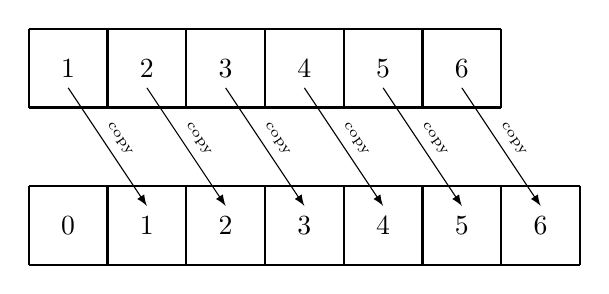
\begin{tikzpicture}
            \draw[thick] (0,0) grid ++(6,1);
            \draw[thick] (0,-2) grid ++(7,1);

            \foreach[evaluate={int(\i+1)} as \j] \i in {0,...,5} {
                \node at (\i + 0.5,0.5) {\j};
                \node at (\i + 1.5,-1.5) {\j};
                \draw[-latex] (\i + 0.5,0.25) -- (\i + 1.5,-1.25) node[midway,sloped,font=\tiny,above] {copy};
            }

            \node at (0.5,-1.5) {0};
        \end{tikzpicture}
    \end{center}
    \vskip4mm
    \structure{Algorithm}
    \begin{itemize}
        \item Create new array with larger size
        \item Copy all elements
        \item $O(n)$
    \end{itemize}
\end{frame}

\begin{frame}
    \frametitle{Add to Front of Linked List}
    \begin{center}
        \begin{tikzpicture}[link/.style={thick,-latex}]
            \foreach[evaluate={(\i - 1) * 1.5} as \x] \i in {1,...,5} {
                \coordinate (p\i) at (\x,0);
                \llnode[position={p\i},size=0.5cm,value=\i]
            }

            \foreach[evaluate={(\i - 1) * 1.5} as \x] \i in {1,...,4} {
                \draw[-latex] ($ (p\i) + (0.75,0.25) $) -- ++(0.75,0);
            }

            \coordinate (p0) at ($ (p1) + (0,-1.5) $);
            \llnode[position=p0,size=0.5cm,value=0]
            \draw[-latex] ($ (p0) + (0.75,0.25) $) -- ($ (p1) + (0.5,0) $);
        \end{tikzpicture}
    \end{center}
    \vskip4mm
    \structure{Algorithm}
    \begin{itemize}
        \item Create new node
        \item Have it point to the (originally) first node
        \item $O(1)$
    \end{itemize}
\end{frame}
